\documentclass[aspectratio=169]{beamer}
\usetheme{metropolis}
% \usetheme{gotham}
% \useoutertheme[
%   progressbar position=foot,   % 进度条位置:foot/head/none
%   progressbar style=rectangle, % 样式:rectangle/rounded box/circle
%   numbering=totalframenumber   % 页码样式:none/framenumber/totalframenumber
% ]{gotham}

\usefonttheme{professionalfonts} % 使用系统/自定字体


% === 字体设置 ===
\usepackage[UTF8,scheme=plain,fontset=none]{ctex}
\setCJKmainfont{Source Han Serif CN}[BoldFont={Source Han Serif CN Bold}]
\setCJKsansfont{Source Han Sans CN}[BoldFont={Source Han Sans CN Bold}]
% \setCJKmonofont{Sarasa Mono CN}


% beamer 已加载 hyperref;加 unicode 以支持中文书签
\hypersetup{unicode}

% define paragraph
\providecommand{\paragraph}[1]{\smallskip\textbf{#1}\par}

% 常用包
\usepackage{longtable,booktabs}
\usepackage{amsmath,amssymb}
\usepackage{graphicx}
\graphicspath{{.}{./figs/}{./images/}{./images_in_paper/}}
\usepackage{caption}
\usepackage{subcaption}
\usepackage{float}
\usepackage{svg}
\usepackage{booktabs}
\usepackage{array}
\usepackage{threeparttable}

% 超链接(beamer 已加载 hyperref,这里只补选项)
% \hypersetup{unicode=true}

% 编号风格
\setbeamertemplate{caption}[numbered]
\setbeamertemplate{caption label separator}{.}

\title{从时域到频域:基于多分支CNN网络的AI音频检测模型}
\author{NKUMMF2025138}
\date{\today}


%---Document Begins---
\begin{document}

\begin{frame}
  \titlepage
\end{frame}


\begin{frame}{摘要}
\small
\begin{itemize}
  \item 问题一:
    \begin{itemize}
      \item 从\textbf{时域、频域及声学统计量}等角度提取 11 类特征,多分支并行融合判别;
      \item 基于\textbf{多分支卷积神经网络(Multi-Branch CNN)}的端到端 AI 音频检测与评分模型;
    \end{itemize}

  \item 问题二:
    \begin{itemize}
      \item 设计\textbf{分支探针机制},依据各分支判别准确率加权,构建可解释的 AI 痕迹评分;
    \end{itemize}

  \item 问题三:
    \begin{itemize}
      \item 引入\textbf{频谱均衡、高频注入、环境噪声混入}等扰动测试模型鲁棒性;
    \end{itemize}
  \vspace{0.8cm}
  \item 模型在测试集上准确率达 \textbf{89.24\% $\pm$ 0.43\%},在多种扰动下表现稳健,具\textbf{低计算开销与良好可扩展性}。
\end{itemize}
\end{frame}


\section{判别模型的建立与求解}
% \subsection{模型假设}
% \begin{frame}[fragile,allowframebreaks]{模型假设}
% \small
% \begin{enumerate}
%     \item 人工标注的“真人/AI”标签总体正确率较高;
%     \item 在选定的分析窗口($20$s)内,音频的统计特性近似平稳,从而帧级特征的统计聚合是有效的。
% \end{enumerate}
% \end{frame}
%
% \subsection{数据处理}
% \begin{frame}[fragile,allowframebreaks]{数据处理}
%   \small
%   \begin{enumerate}
%     \item{代码中首先将输入文件转码为 WAV 格式}
%     \item{采用音频处理领域常用的 $22050$ Hz 采样率对输入音频进行统一解码与重采样}
%     \item{在特征提取流程中,原始歌曲首先被切分为 20 秒长度的片段}
%   \end{enumerate}
% 在此基础上,本文提取了表~\ref{tab:audio-features} 中所列的多种时域、频域及声学特征,涵盖能量变化、频谱形状、谐波结构及共振峰等方面的信息。
% \end{frame}
\subsection{特征说明}
\begin{frame}{特征说明}
\begin{table}
  \centering
  \begin{tabular}{lll}
    \toprule
    特征名称 & 维度 & 特征类型 \\
    \midrule
    rms       & (1, 862)   & 时域能量 \\
    zcr       & (1, 862)   & 时域变化 \\
    hjorth    & (3, 1)     & 全局统计 \\
    log\_mel  & (128, 862) & 频域谱图 \\
    mfcc      & (13, 862)  & 声学特征 \\
    centroid  & (1, 862)   & 频谱形状 \\
    contrast  & (7, 862)   & 频谱对比度 \\
    flatness  & (1, 862)   & 频谱形状 \\
    f0        & (1440,)    & 音高曲线 \\
    hnr       & (1998,)    & 声学质量 \\
    formant   & (3, 2000)  & 共振峰 \\
    \bottomrule
  \end{tabular}
  \caption{各特征的名称、维度及类型}\label{tab:audio-features}
\end{table}
\end{frame}


\subsection{模型建立}
\begin{frame}{模型建立}
% 本研究构建了一个多分支卷积神经网络(Multi-Branch CNN),用于融合处理多种类型的音频特征,
% 从而实现对 AI 生成音频的准确识别。整体网络结构如下图所示,模型共由五个输入分支构成,
% 分别对应不同特征类型,并通过特征融合实现最终的二分类判别。
  \vspace{0.2cm}
\begin{figure}[h]
    \centering
    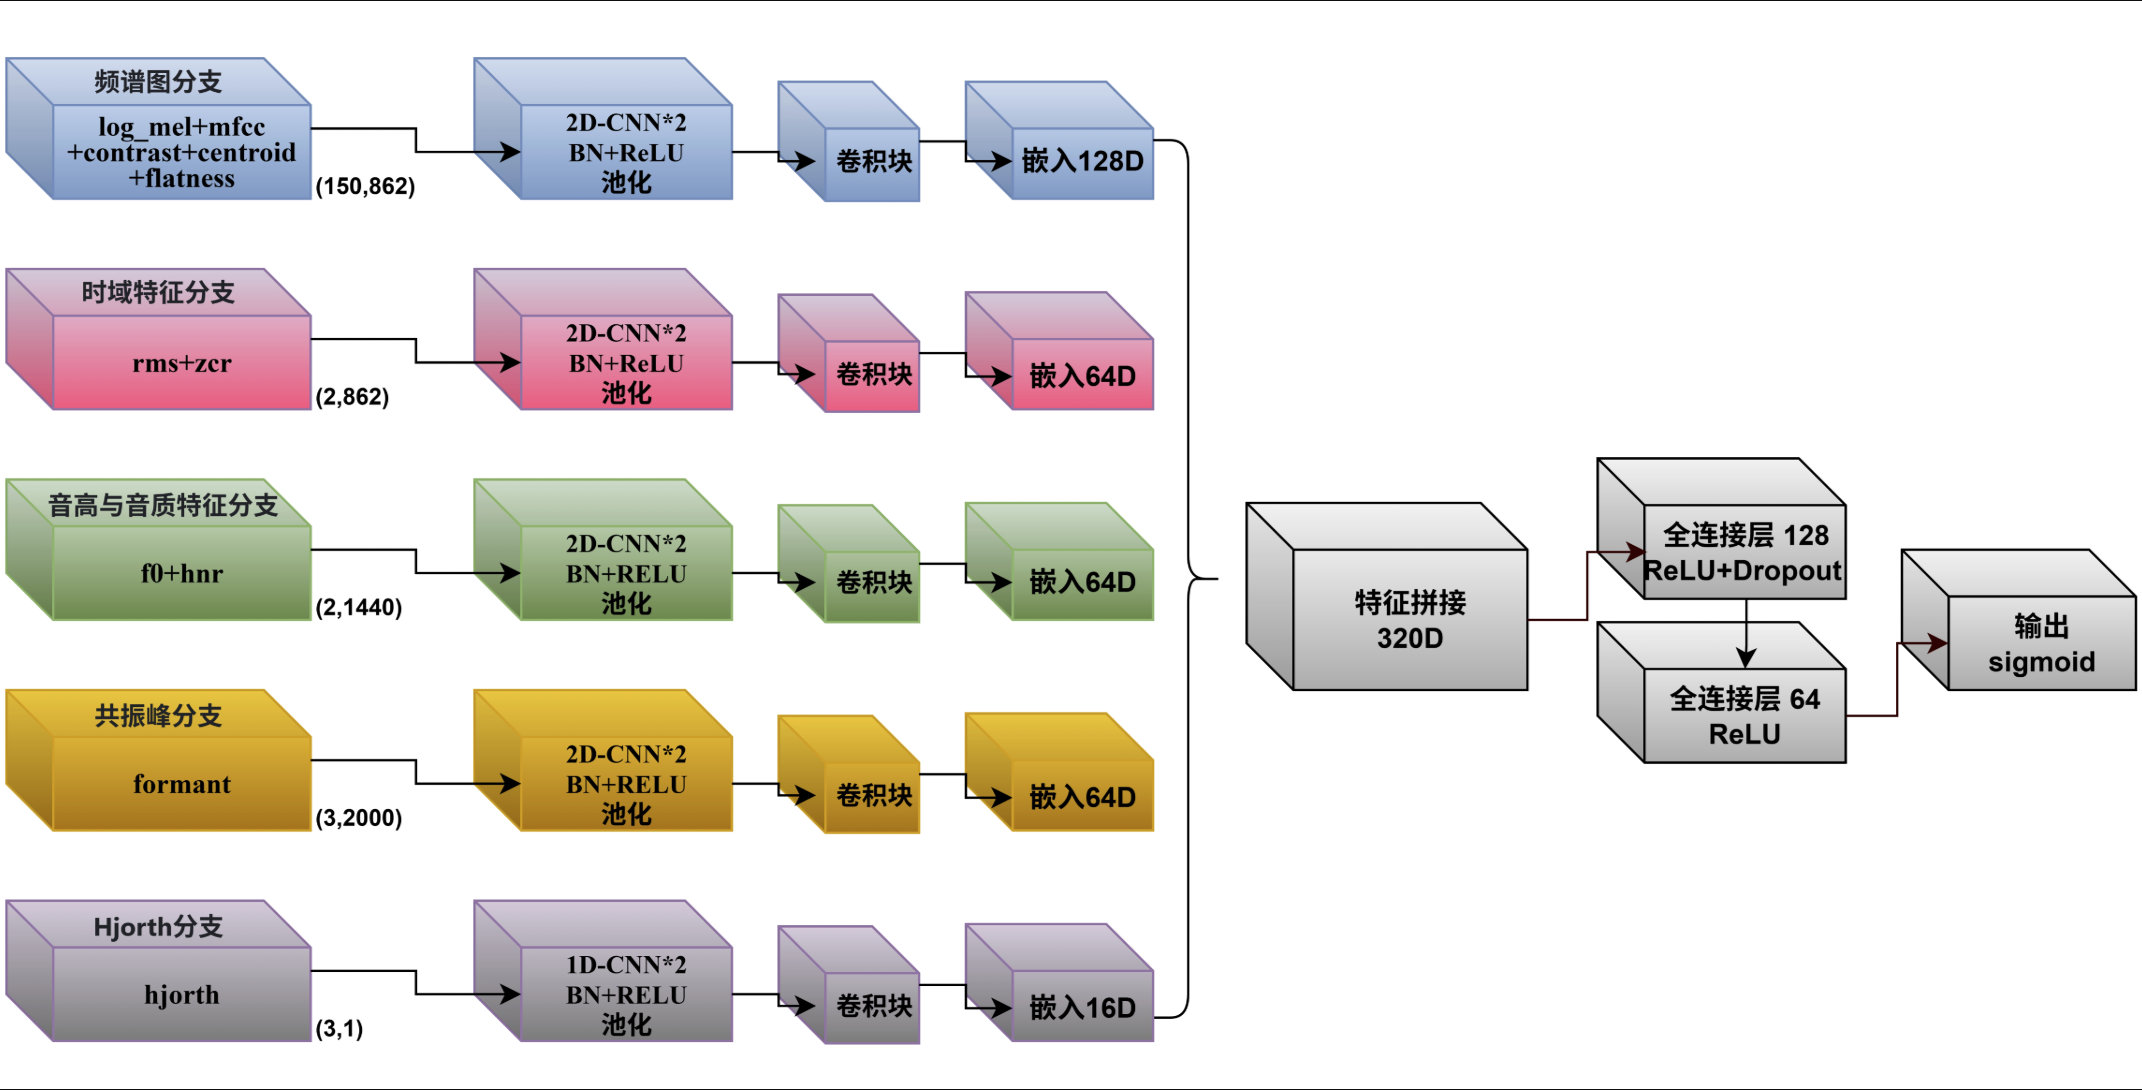
\includegraphics[width=0.75\linewidth]{images_in_paper/model.png}
    \caption{多分支CNN示意图}
    \label{fig:model}
\end{figure}

\end{frame}

% \begin{frame}[fragile,allowframebreaks]{模型建立}
\begin{frame}{模型建立}
\begin{table}[h]
  \centering
  \small
  \resizebox{\textwidth}{!}{%
  \begin{tabular}{lll}
    \toprule
    \textbf{分支名称} & \textbf{输入特征} & \textbf{处理与输出} \\
    \midrule
    频谱图分支(Spectrogram) & log\_mel, mfcc, contrast, centroid, flatness & 2D CNN 提取时频模式 → GAP → 128 维表示 \\[2pt]
    时域分支(Time-Domain) & rms, zcr & 1D CNN 提取时间结构 → 64 维向量 \\[2pt]
    音高与音质分支(Pitch \& Quality) & f0, hnr & 1D CNN 建模调型与音质 → 64 维向量 \\[2pt]
    共振峰分支(Formant) & formant & 1D CNN 处理时间序列 → 64 维向量 \\[2pt]
    Hjorth 参数分支(Hjorth Param.) & hjorth (Activity, Mobility, Complexity) & 两层全连接 → 16 维表示 \\
    \bottomrule
  \end{tabular}%
  }
  \caption{多分支特征处理结构概览}
  \label{tab:branch-structure}
\end{table}

% 五个分支提取的特征向量分别为:128维(频谱图)、64维(时域)、64维(音高音质)、64维(formant)与16维(hjorth),合并后得到一个 $336$ 维的全局音频表征。该向量随后输入至全连接分类器,包含一层隐藏层(64单元),使用 ReLU 激活与 Dropout 防止过拟合,最终输出一个概率值,判定音频是否为 AI 生成。
\end{frame}


\subsection{结果分析}
\begin{frame}{结果分析}
\begin{figure}[htb]
  \centering
  \begin{subfigure}{0.48\linewidth}
    \centering
    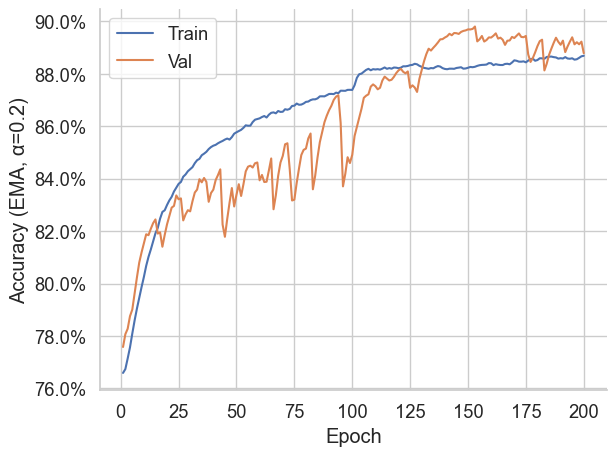
\includegraphics[width=\linewidth]{images_in_paper/acc_train_val.png}
    \caption{准确率(Train vs Val)}
    \label{fig:acc}
  \end{subfigure}\hfill
  \begin{subfigure}{0.48\linewidth}
    \centering
    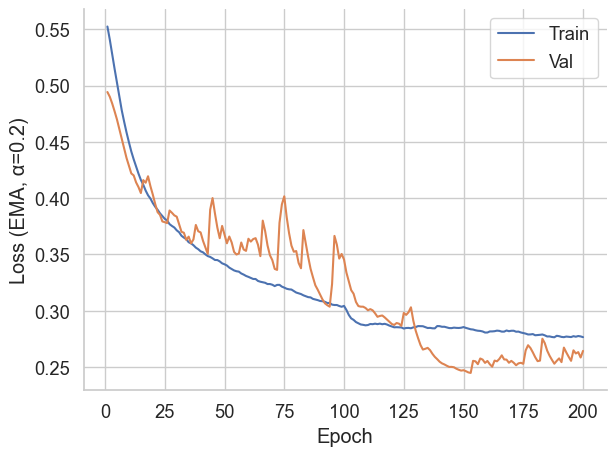
\includegraphics[width=\linewidth]{images_in_paper/loss_train_val.png}
    \caption{损失(Train vs Val)}
    \label{fig:loss}
  \end{subfigure}
  \caption{训练过程的准确率与损失对比}
  \label{fig:acc-loss}
\end{figure}
\end{frame}

% \begin{frame}[fragile,allowframebreaks]{结果分析}
%
%   训练损失呈单调递减趋势,最终趋近于0.27;
%
%   训练集准确率从\textbf{76.5\%}持续上升并最终收敛于\textbf{88.5\%}左右,
%
%   验证集准确率和损失虽经历多次波动,但最终趋于稳定,
%   分别在\textbf{89\%-90\%}和\textbf{0.25-0.26}之间。
%
%   上述结果表明模型训练稳定,未出现过拟合迹象。
%   这说明多分支特征融合结构在提取不同维度音频信息时具有较好的\textbf{泛化能力},
%   能够有效捕捉AI生成音乐与人类创作音乐的差异特征。
%
% \end{frame}

\subsection{消融实验}
\begin{frame}[fragile,allowframebreaks]{消融实验}
为探究各输入分支在多分支 CNN 模型中的贡献度,本研究设计了消融实验,
通过控制不同分支的启用/关闭状态,评估其对模型分类精度的影响。
具体而言,我们分别在以下三种设置下进行测试:
\begin{itemize}
  \item 全分支开启;
  \item 单独关闭某一分支,其余保持开启;
  \item 单独开启某一分支,其余全部关闭。
\end{itemize}
\end{frame}

\begin{frame}[allowframebreaks]{消融实验}
\scriptsize
\begin{longtable}{cccccc}
\caption{消融实验结果(准确率 \%)\label{tab:ablation}}\\
\toprule
频谱图分支 & 时域分支 & 音高与音质分支 & 共振峰分支 & Hjorth 参数分支 & 准确率 \\
\midrule
\endfirsthead
\caption[]{消融实验结果(续)}\\
\toprule
频谱图分支 & 时域分支 & 音高与音质分支 & 共振峰分支 & Hjorth 参数分支 & 准确率 \\
\midrule
\endhead
\bottomrule
\multicolumn{6}{r}{\footnotesize 续下页…}\\
\endfoot
\bottomrule
\multicolumn{6}{l}{\footnotesize 注:1 表示该 CNN 分支传入真实特征张量,0 表示相同形状的全零张量。}\\
\endlastfoot
1 & 1 & 1 & 1 & 1 & 89.24\% \\
0 & 1 & 1 & 1 & 1 & 29.87\% \\
1 & 0 & 1 & 1 & 1 & 79.20\% \\
1 & 1 & 0 & 1 & 1 & 88.77\% \\
1 & 1 & 1 & 0 & 1 & 88.40\% \\
1 & 1 & 1 & 1 & 0 & 89.10\% \\
1 & 0 & 0 & 0 & 0 & 77.87\% \\
0 & 1 & 0 & 0 & 0 & 30.02\% \\
0 & 0 & 1 & 0 & 0 & 47.76\% \\
0 & 0 & 0 & 1 & 0 & 50.67\% \\
0 & 0 & 0 & 0 & 1 & 25.20\% \\
\end{longtable}

\end{frame}


\begin{frame}[fragile,allowframebreaks]{消融实验}
虽然消融实验能够衡量各分支在整体判别任务中的贡献度,但这种方法仍存在一定局限性:  
\begin{itemize}
  \item \textbf{无法独立量化单分支判别能力}
  \item \textbf{分支间存在互补与冗余效应}
  \item \textbf{评估结果依赖当前模型权重分布}
  \item \textbf{未能刻画特征在不同类型样本上的贡献差异}
\end{itemize}
针对以上不足,我们在后续模型中引入了分支探针机制,使每个分支能够在保持原有多分支协作的同时,
\textbf{单独}完成二分类任务,从而获得更客观、细粒度的特征贡献评估结果。

\end{frame}

% \begin{frame}[fragile,allowframebreaks]{消融实验}
% 虽然消融实验能够衡量各分支在整体判别任务中的贡献度,但这种方法仍存在一定局限性:  
% \begin{itemize}
%   \item \textbf{无法独立量化单分支判别能力}:在消融实验中,关闭某一分支时其特征被替换为零向量,其余分支仍参与决策,因此所得精度下降值只是间接反映该分支的重要性,而非其独立完成任务的真实表现。  
%   \item \textbf{分支间存在互补与冗余效应}:不同分支特征可能存在高度相关性,关闭一个分支后,其信息可能部分被其他分支补偿,导致重要性被低估;反之,如果多个分支特征冗余,关闭其中一个分支对结果影响可能被夸大。  
%   \item \textbf{评估结果依赖当前模型权重分布}:消融实验是在固定训练好的多分支模型上进行的,权重分布已经针对多特征融合进行了优化,单分支输入下的表现可能不能代表该分支在独立训练时的潜力。  
%   \item \textbf{未能刻画特征在不同类型样本上的贡献差异}:消融实验只给出整体平均精度,而没有分析分支在不同类别、不同难度样本上的表现差异,限制了对特征适用性的理解。  
% \end{itemize}
% 针对以上不足,我们在后续模型中引入了分支探针机制,使每个分支能够在保持原有多分支协作的同时,单独完成二分类任务,从而获得更客观、细粒度的特征贡献评估结果。
%
% \end{frame}



\section{评分机制}
\subsection{定义评分公式}
\begin{frame}{评分公式的定义}
受消融实验结果的启发,为了细化模型的评价指标,我们改进了多分支CNN网络,
为每个分支添加了一个由线性层和\texttt{Sigmoid}函数构成的\textbf{探针头结构}。

对于一段音频,每个分支的探针都可以独立判断该音频是否为AI生成,并输出\textbf{分类概率}。
\end{frame}

\begin{frame}[fragile,allowframebreaks]{评分规则}
% ========== 公式:评分规则 ==========
\paragraph{评分规则} 记各分支探针头给出的“音频为AI生成”的概率为
$p_i\in[0,1]$,则作品的综合评分(AI痕迹强度)定义为
\begin{equation}
    S \;=\; \sum_{i} \omega_i\, p_i \;\in\;[0,1],
    \label{eq:ai_score}
\end{equation}
其中 $\omega_i$ 为分支的评分权重。$S$ 越大表示该音频越可能为 AI 生成。
\end{frame}

\begin{frame}{分支权重的确定}
在综合各分支结果为音乐作品打分时,我们以各探针头单独决策时的\textbf{准确率}为依据,
确定了各分支的评分权重。

% ========== 公式:权重确定 ==========
设各分支探针在独立判别(AI/非AI)下的准确率
$acc_i,i\in\{\text{spec,time,prosody,formant,hjorth}\}$。

为避免随机猜测带来的偏置,先做机会校正(chance-corrected)并归一化:

\begin{equation}
    \omega_i \;=\; \frac{acc_i-0.5}{\sum_j (acc_j-0.5)},\qquad 
    \sum_i \omega_i = 1.
    \label{eq:branch_weight}
\end{equation}
\end{frame}


\begin{frame}[fragile,allowframebreaks]{实验结果}
% ========== 结果与分析(含表格) ==========

\begin{table}[htbp]
\centering
\caption{分支探针头独立预测准确率及由此推导出的归一化权重}
\label{tab:probe-acc-weight}
\begin{tabular}{lcc}
\toprule
分支(Branch) & 准确率 $a_i$ & 权重 $w_i$ \\
\midrule
spec(频谱图)      & 0.7725 & 0.1987 \\
time(时域)        & 0.7834 & 0.2067 \\
prosody(音高音质) & 0.7718 & 0.1982 \\
formant(共振峰)   & 0.7717 & 0.1981 \\
hjorth(Hjorth)    & 0.7718 & 0.1982 \\
\midrule
主分类器(参考)    & 0.8924 & -- \\
\bottomrule
\end{tabular}
\end{table}
\end{frame}


\subsection{结果与分析}
%commentHere
% \begin{frame}[fragile,allowframebreaks]{分析讨论}
% \paragraph{探针准确率与权重} 
% % 表~\ref{tab:probe-acc-weight} 
% % 汇总了主分类器与各分支探针的独立准确率以及依据式(1)计算得到的分支权重。
% % 可以看到,\texttt{time} 分支(时域特征)在单分支判别中的准确率最高($78.34\%$),
% % 因此在综合评分中获得了略高的权重($0.2067$);
% % 其余四个分支的准确率非常接近(约 $77.17\%\sim77.25\%$),
% % 对应的权重也基本均衡(约 $0.198$)。
% % 这种结果与我们在问题一中对多源特征互补性的观察一致:
% % 频谱类与声学统计特征在区分 AI 音频时具有相近而可互补的判别力。
%
% 从独立判别能力看,各分支探针准确率集中在 $77\%\sim78\%$ 区间,
% 说明不同模态特征(时域、频域、声学统计与共振峰)在本任务上均具较强的区分信息,
% 且不存在明显的“短板”分支。
% 各分支探针的准确率相比于消融实验结果(表~\ref{tab:ablation})多数分支有较高提升,
% 进一步证实了加入探针头对模型进行微调的必要性。
%
% 综合评分采用式\ref{eq:ai_score}的线性加权后,可在推理阶段以显式、
% 可解释的方式衡量各分支对最终结论的贡献。
%
% 主分类器的总体准确率为 $89.24\%$,显著高于任一单分支探针,
% 验证了多特征融合的有效性;而探针权重的近似均衡分布则为后续的可解释分析提供了稳定基线。
% \end{frame}



\section{鲁棒性分析}
\begin{frame}[fragile,allowframebreaks]{鲁棒性分析}
  \begin{itemize}
    \item 构造扰动
    \item 分析扰动实验结果
    \item 结合\textbf{数据流}进行归因分析
  \end{itemize}
\end{frame}

\subsection{扰动构造}
\begin{frame}[fragile,allowframebreaks]{扰动构造}
从模型和数据两个角度入手,构造扰动:
\begin{enumerate}
\item \textbf{模型角度:}修改音频,对模型特征进行直接干扰
  \begin{itemize}
    \item \textbf{时域分支:} 轻度动态压缩、滤波器、相位扰动;
    \item \textbf{频域分支:} EQ频段调节;
    \item \textbf{类共振峰分支:} 对常见人声频段进行增益/衰减;
    \item \textbf{全局统计分支:} 局部加速/减速,改变节奏特征;
    \item \textbf{音高与谐噪比分支:} 对音高作 $\pm 0.15$ semitone 平移,加入低幅白噪声。
  \end{itemize}

\item \textbf{数据角度:}音轨合并扰动\\
  将原始音频与自然环境噪声片段(如 \emph{city park, forest, rain})按不同响度比例混合,构造更具真实感的样本。
\end{enumerate}

\end{frame}

\subsection{实验方案}
\begin{frame}[fragile,allowframebreaks]{扰动实验结果及分析}

对真实标签为"AI生成"的音频施加前述两类扰动,构造测试集,分别计算:
\[
S = \text{加权融合评分}, \quad \texttt{prob\_main} = \text{主分类概率}
\]
  每类扰动设置 \texttt{mild}、\texttt{medium}、\texttt{strong} 三档强度,
  并统一归一化 RMS 以消除响度影响。
\end{frame}

% \begin{frame}[fragile,allowframebreaks]{扰动实验结果及分析}
%
% \textbf{分析流程:}
%
% \begin{enumerate}
%   \item \textbf{扰动集划分:}
%   \begin{itemize}
%     \item 细粒度特征通道扰动:包括 RMS/相位扰动、倾斜式 EQ、窄带峰值 EQ、共振峰微调、节奏微变、音高与谐噪比调整;
%     \item 频率域参数均衡器扰动:多组中心频率、增益与品质因数组合的窄带或宽带 \emph{peaking} EQ;
%     \item 音轨合并扰动:与环境音(城市、公园、雨声)按不同比例混合。
%   \end{itemize}
%   每类扰动设置 \texttt{mild}、\texttt{medium}、\texttt{strong} 三档强度,
%   并统一归一化 RMS 以消除响度影响。
%
%   \vspace{0.4em}
%   \item \textbf{推理与统计:}\\
%   对每个扰动子集输入模型推理,计算:
%   \[
%   \text{均值}(\texttt{prob\_main}), \quad \text{均值}(S), \quad
%   \text{相对降幅}, \quad \text{标准差变化}
%   \]
%   以量化扰动对检测性能的影响。
%
%   \vspace{0.4em}
%   \item \textbf{结果汇总与对比:}\\
%   比较主分类头与融合评分在抗扰动能力上的差异,
%   重点关注:
%   \begin{itemize}
%     \item 高频注入(spectral tilt / EQ)
%     \item 环境噪声混入(noise mix)
%     \item 共振峰微调(formant shift)
%   \end{itemize}
%   分析模型预测稳定性与置信度变化规律。
% \end{enumerate}
%
% \end{frame}
%
% \subsection{鲁棒性结果}
\begin{frame}[fragile,allowframebreaks]{不同扰动类型下的鲁棒性表现}
下表汇总了五组混淆效果较大的实验结果。
\small
\begin{table}[h]
\centering
\caption{不同扰动类型下主分类概率与综合评分均值对比}
\label{tab:family-stats}
\resizebox{\textwidth}{!}{%
\begin{tabular}{lcccc}
\toprule
扰动方式 & 示例 & 样本数 & $\texttt{prob\_main}$ 均值 & $S$ 均值 \\
\midrule
\textbf{comboAll}       & 多种扰动叠加版本                 & 1  & 0.764 & 0.776 \\
\textbf{pitchHNR}       & 音高调整 + 白噪音注入              & 1  & 0.659          & 0.757 \\
\textbf{specEQ}         & EQ              & 7  & 0.604          & 0.727 \\
\textbf{highFreqInject} & 高频注入(HI)                   & 8  & 0.461          & 0.667 \\
\textbf{ambientNoise}   & 环境噪声混入(雨声、森林、城市) & 4  & 0.422          & 0.671 \\
\bottomrule
\end{tabular}
}
\end{table}
\end{frame}
%commentHere
% \begin{frame}[fragile,allowframebreaks]{不同扰动类型下的鲁棒性表现}
% % \vspace{0.8em}
% \textbf{分析:}
% \begin{itemize}
%   \item \textbf{总体表现:} 多种扰动叠加(\texttt{comboAll})在主分类概率和综合评分上仍保持在 0.76 以上,模型具备较强鲁棒性;
%   \item \textbf{轻度扰动:} 音高与谐噪比调整(\texttt{pitchHNR})对性能影响较小,综合评分 $S=0.757$;
%   \item \textbf{中等扰动:} 频谱均衡/倾斜(\texttt{specEQ})使主分类概率下降至 0.604;
%   \item \textbf{高风险扰动:} 高频注入与环境噪声混入显著降低模型输出置信度,\texttt{prob\_main} 分别降至 0.461 和 0.422;
%   \item \textbf{综合结论:} 环境噪声在较低响度比例下即可破坏时域与频域模式,是当前模型鲁棒性提升的关键方向。
% \end{itemize}
%
% \end{frame}

\subsection{归因分析:分支数据流与扰动敏感性的关联}
\begin{frame}[fragile,allowframebreaks]{归因分析:分支数据流特征与扰动敏感性的关联}

\textbf{目的:}  
探究检测器在不同分支上的数据流特征与其对扰动的敏感性之间的关系。

\vspace{0.6em}
\textbf{方法:}
\begin{itemize}
  \item 对各 CNN 分支的嵌入空间(即输入全连接层前的一维张量)进行降维可视化;
  \item 分析各分支在嵌入空间中的类别可分性;
  \item 采用 AUC、ACC、Fisher 比率与 logit 统计量量化每个分支对最终决策的贡献。
\end{itemize}
\end{frame}

% commentHere
% \begin{frame}[fragile,allowframebreaks]{归因分析:分支表征与扰动敏感性的关联}
% % \vspace{0.6em}
% \textbf{发现要点:}
% \begin{enumerate}
%   \item \textbf{时域分支更“可分”}:AI 音频在能量包络与瞬态结构维度上形成独立簇;
%   \item \textbf{共振峰分支更“缠绕”}:formant 嵌入分布交叠,区分度较低;
%   \item PCA 投影虽线性可分性有限,但沿第一主轴可观察到标签渐变。
% \end{enumerate}
% \end{frame}

\begin{frame}{归因分析:分支数据流特征与扰动敏感性的关联}
\begin{figure}
  \centering
  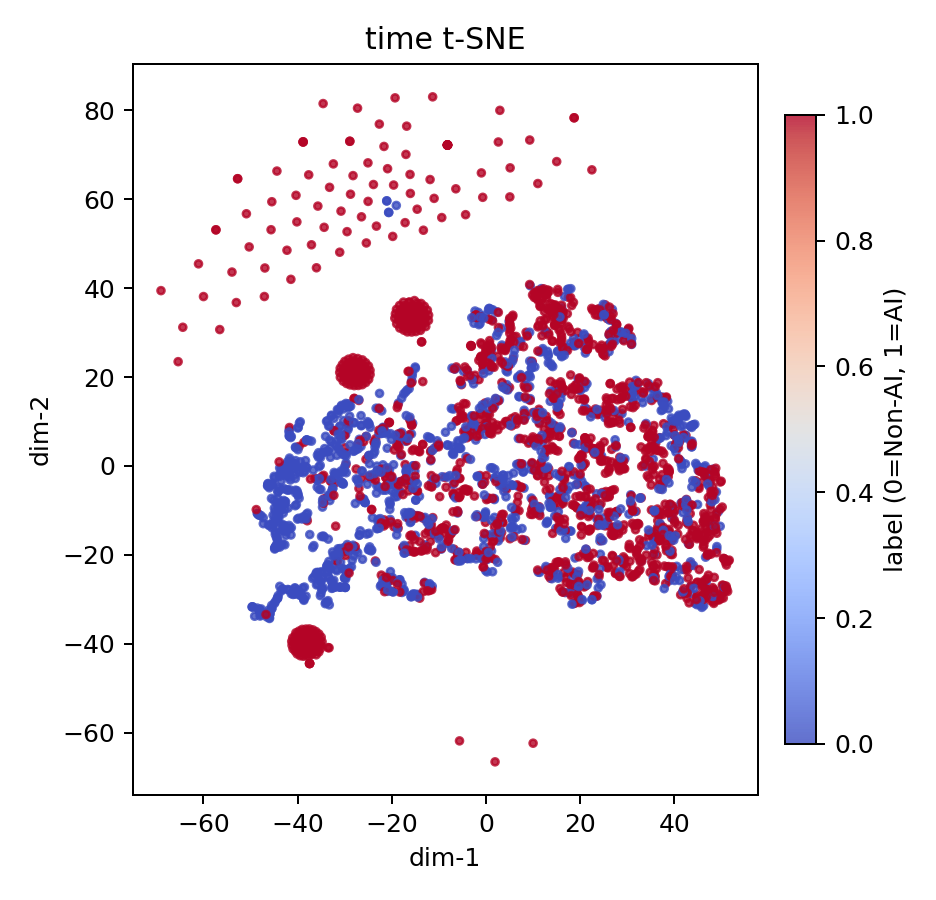
\includegraphics[width=0.45\linewidth]{images_in_paper/embed_time_tsne.png}
  \hfill
  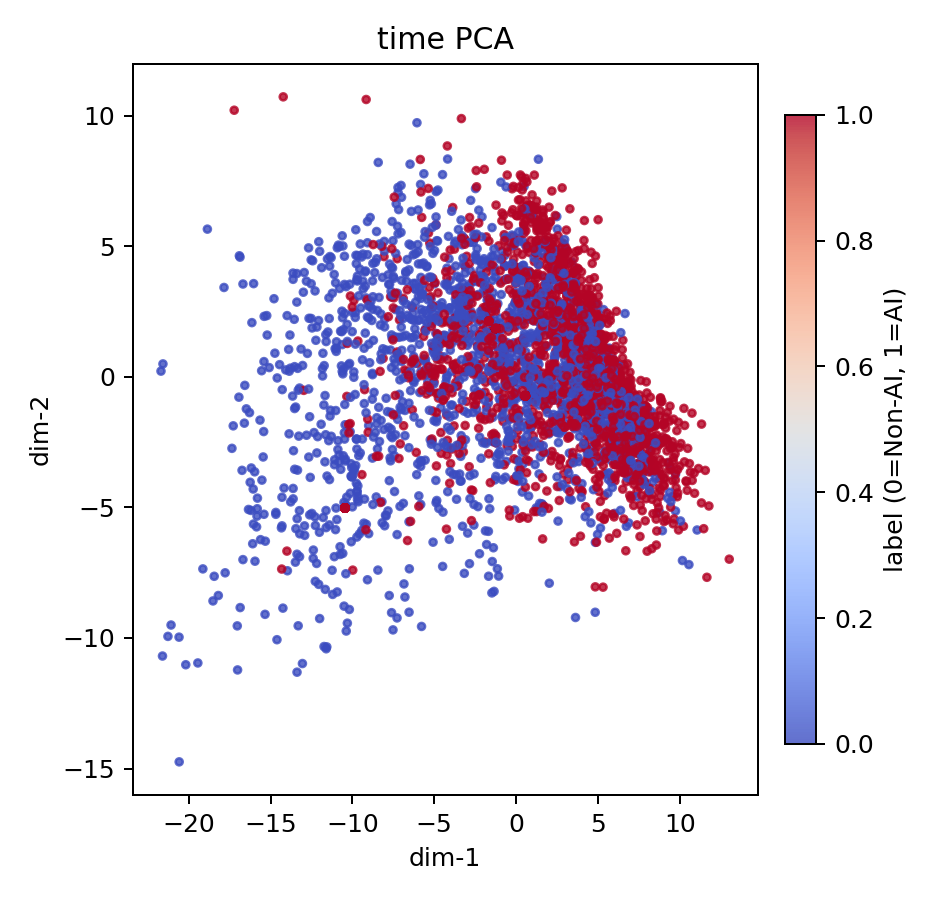
\includegraphics[width=0.45\linewidth]{images_in_paper/embed_time_pca.png}
  \caption{时域分支嵌入可视化:t-SNE(左)与 PCA(右)。}
  \label{fig:time_tsne_pca}
\end{figure}
\end{frame}


% \begin{frame}[fragile,allowframebreaks]{归因分析:共振峰分支嵌入特征}
%
% \textbf{观察:}  
% formant 分支在嵌入空间中的红蓝标签高度交织,仅在部分区域出现局部聚集。
%
% \vspace{0.6em}
% \textbf{分析要点:}
% \begin{itemize}
%   \item 整体频谱包络不足以稳定区分所有 AI 样式;
%   \item 局部区域(“岛状簇”)反映特定风格的 AI 样本,
%         例如使用相似声道或共振峰模板的生成模型;
%   \item 与时域分支相比,formant 分支特征的全局可分性显著较低,
%         但具备一定的局部判别力。
% \end{itemize}
% \end{frame}

\begin{frame}{归因分析:共振峰分支嵌入特征}
% \vspace{0.6em}
\begin{figure}
  \centering
  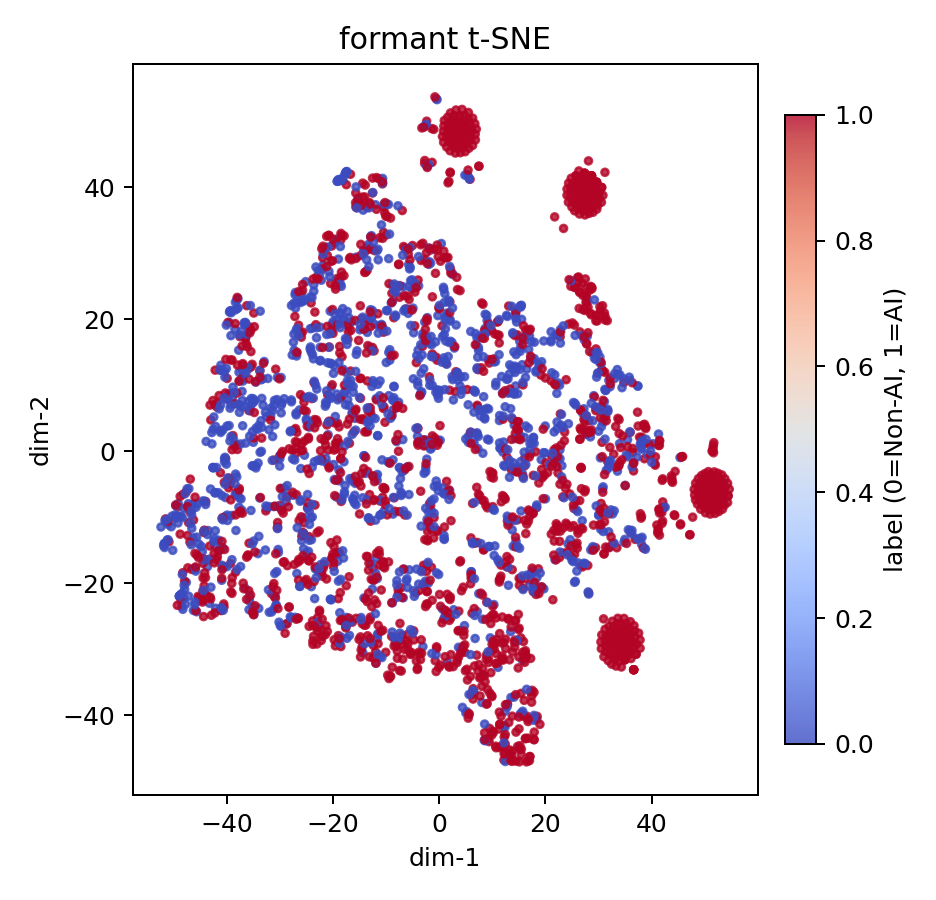
\includegraphics[width=0.45\linewidth]{images_in_paper/embed_formant_tsne.png}
  \hfill
  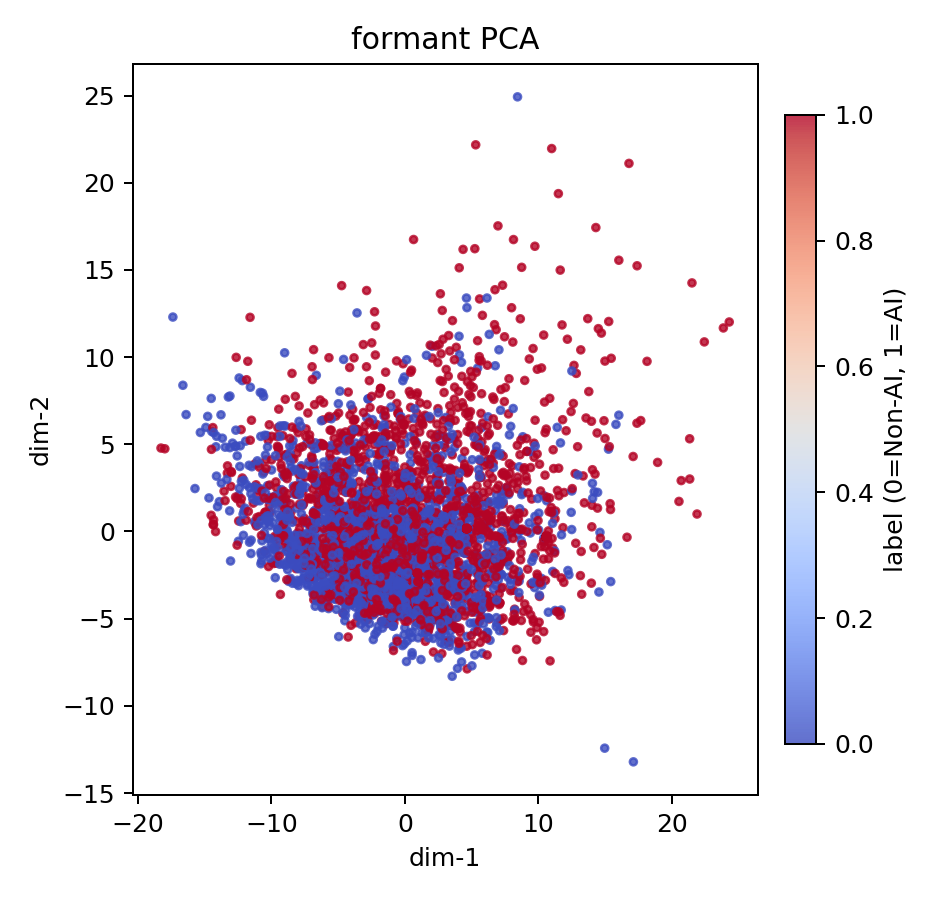
\includegraphics[width=0.45\linewidth]{images_in_paper/embed_formant_pca.png}
  \caption{formant 分支嵌入可视化:t-SNE(左)与 PCA(右)。}
  \label{fig:formant_embed}
\end{figure}

\end{frame}



\begin{frame}[fragile,allowframebreaks]{量化分析:contrib 指标定义}
\vspace{0.6em}
\textbf{Contribution 指标:}
\begin{itemize}
  \item \textbf{Grad$\times$Input},
    \[
      \mathrm{contrib}_k \approx
      \sum_{j \in \mathcal{I}_k}
      \frac{\partial y}{\partial z_j}\, z_j,
    \]
    其中 $\mathcal{I}_k$ 表示第 $k$ 个分支在拼接向量中的索引集合。
  \item $\mathrm{contrib}_k > 0$ 表示该分支对判决结果具有正向推动作用(倾向于判为 AI),
        $\mathrm{contrib}_k < 0$ 则表示负向作用(倾向于判为非 AI)。
\end{itemize}
\end{frame}

\begin{frame}{量化分析:分支贡献的相关性与对冲关系}
\vspace{0.6em}
\begin{figure}
  \centering
  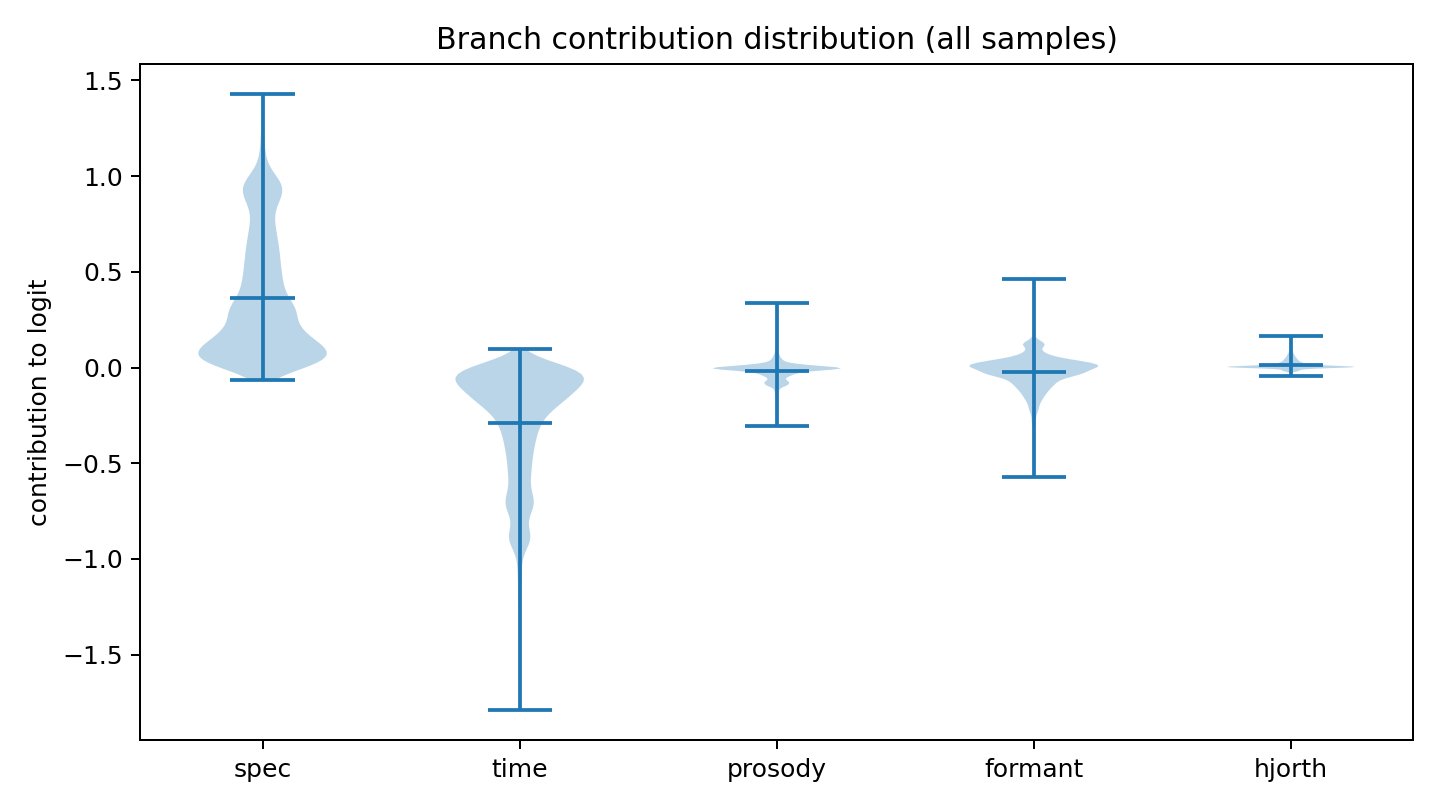
\includegraphics[width=0.75\linewidth]{images_in_paper/contrib_violin_all.png}
  \caption{各分支 logit 贡献的分布(所有样本)。}
  \label{fig:contrib_violin}
\end{figure}

\end{frame}

\begin{frame}{量化分析结果:分支贡献对比}
\begin{figure}
  \centering
  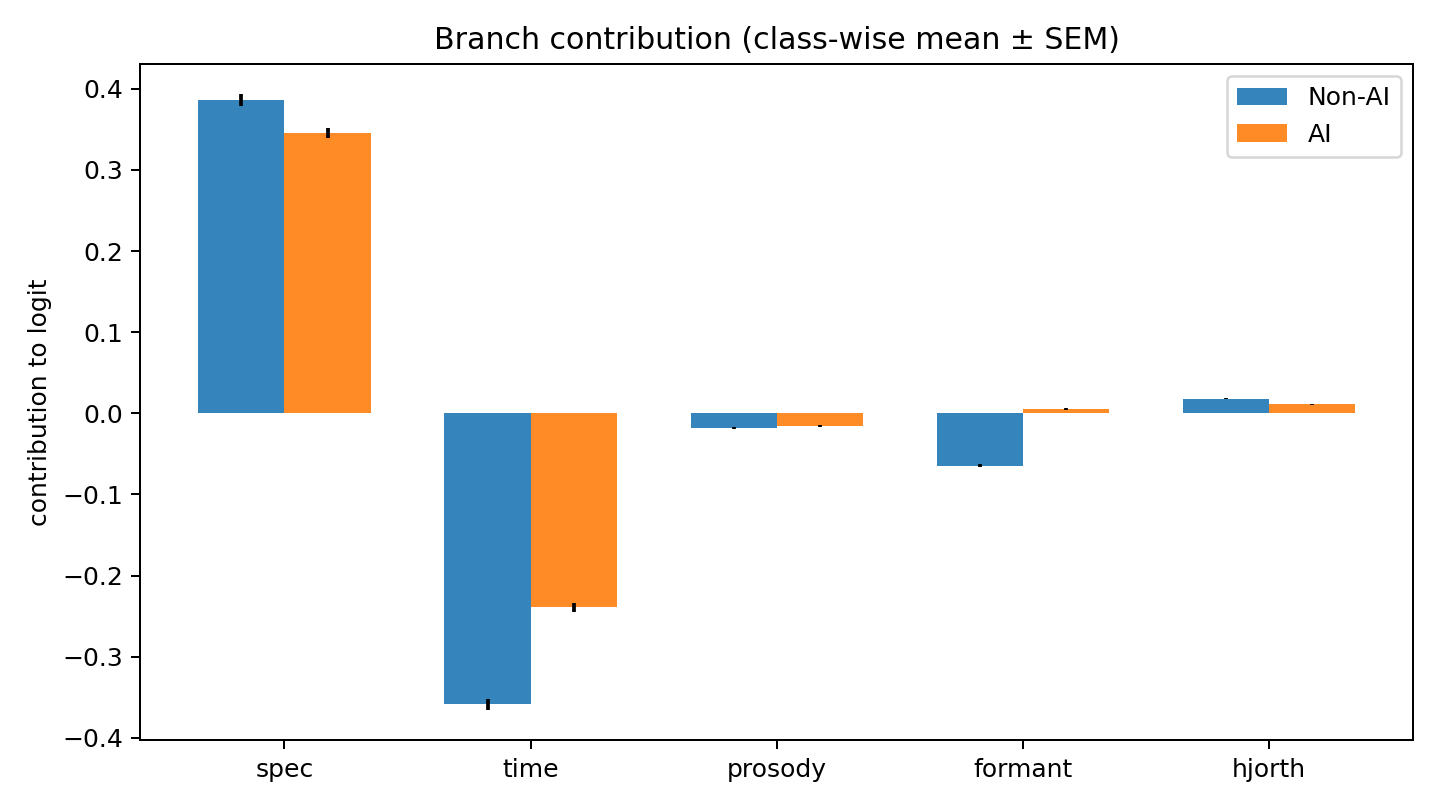
\includegraphics[width=0.7\linewidth]{images_in_paper/contrib_means_by_class.png}
  \caption{各分支在 AI 与非 AI 样本上的平均贡献值(均值±标准误差)。}
  \label{fig:contrib_means}
\end{figure}
\end{frame}

\begin{frame}[fragile,allowframebreaks]{量化分析结果:分支贡献对比}
\textbf{结果概要:}
\begin{itemize}
  \item 图~\ref{fig:contrib_means} 展示了不同分支在 AI 与非 AI 样本上的
        平均贡献值(均值 ± 标准误差);
  \item \texttt{spec} 分支在两类样本中均呈显著\textbf{正贡献},
        推高 AI 判别概率;
  \item \texttt{time} 分支整体为\textbf{负贡献},
        对 AI 判别起抑制作用,且幅度较大;
  \item \texttt{prosody}、\texttt{formant} 与 \texttt{hjorth} 分支的贡献幅度较小,
        表明其对最终判决的直接推动作用有限。
\end{itemize}

\end{frame}


\begin{frame}{量化分析:分支贡献的相关性与对冲关系}
\textbf{相关性分析:}
\begin{itemize}
  \item 计算样本层面的皮尔逊相关系数矩阵;
  \item 结果如图~\ref{fig:contrib_corr} 所示:
    \begin{itemize}
      \item \texttt{spec} 与 \texttt{time} 分支呈显著\textbf{负相关};
      \item 表明它们在多数样本中存在“对冲”关系:
        一个分支推动判为 AI 时,另一个往往抑制;
      \item \texttt{prosody} 与 \texttt{time}、\texttt{formant} 呈\textbf{正相关},
        暗示在部分样本中可能协同作用。
    \end{itemize}
\end{itemize}

\end{frame}

\begin{frame}{量化分析:分支贡献的相关性与对冲关系}
% \vspace{0.5em}
\begin{figure}
  \centering
  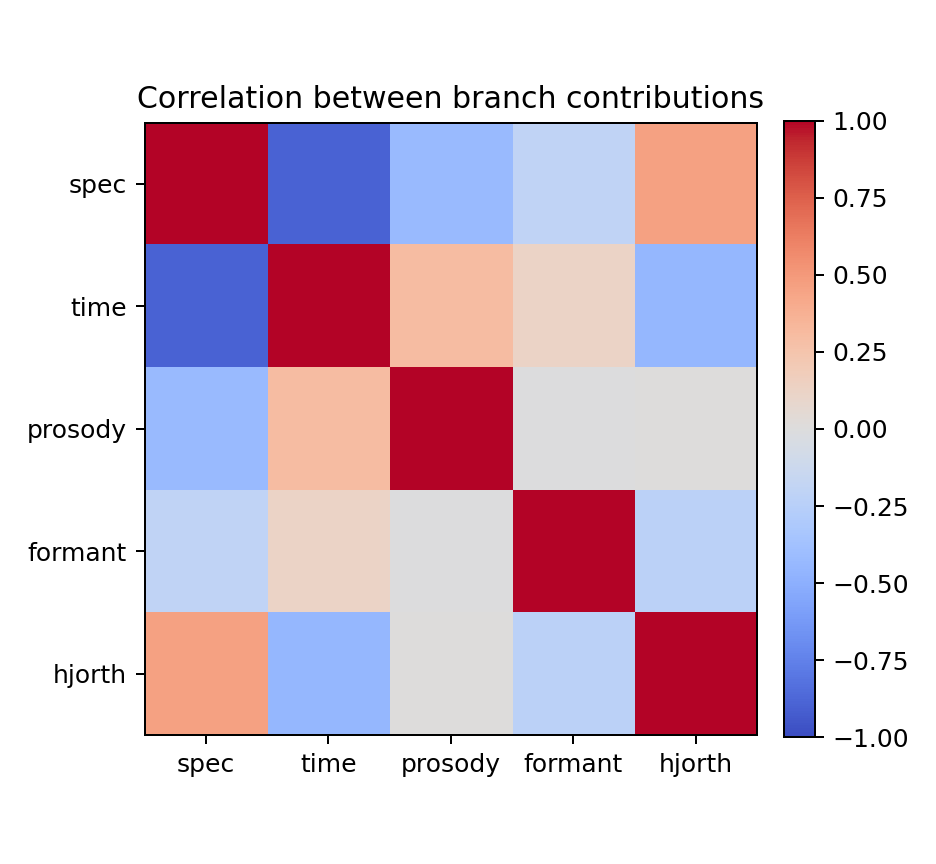
\includegraphics[width=0.5\linewidth]{images_in_paper/contrib_correlation.png}
  \caption{各分支 logit 贡献的相关性矩阵(皮尔逊相关系数)。}
  \label{fig:contrib_corr}
\end{figure}

\end{frame}

%commentHere
% \begin{frame}{量化分析:分支贡献的分布特性}
%
% \textbf{样本级分布:}
% \begin{itemize}
%   \item 图~\ref{fig:contrib_violin} 展示各分支在所有样本上的 logit 贡献分布;
%   \item \texttt{time} 分支:分布跨度最大,从强负到强正均有覆盖;
%         说明其在不同样本中权重差异显著;
%   \item \texttt{spec} 分支:分布集中且整体偏正,
%         表明其稳定推高 AI 判别;
%   \item \texttt{formant} 分支:分布较分散、极端值多,
%         可能在特定声学风格下起关键作用;
%   \item 其他分支(\texttt{prosody}、\texttt{hjorth})贡献较弱,
%         说明其在多数样本中的直接作用有限。
% \end{itemize}
%
% \end{frame}


\begin{frame}[fragile,allowframebreaks]{量化分析:分支判别能力指标定义}

\textbf{目的:}  
评估各分支嵌入的判别能力,分析最终决策对不同分支的依赖性。

\vspace{0.6em}
\textbf{主要指标:}

\begin{itemize}
  \item \textbf{AUC(Area Under the ROC Curve)}
  \begin{itemize}
    \item 表示在所有可能阈值下模型正确区分正负样本的概率;
    \item ROC 曲线越靠近左上角,说明召回率高、误报率低;
    \item AUC 值越接近 1 → 判别能力越强;AUC = 0.5 → 等价于随机猜测;
    \item 图~\ref{fig:roc} 展示各分支的 ROC 曲线。
  \end{itemize}

  \vspace{0.4em}
  \item \textbf{ACC(Accuracy)}
  \begin{itemize}
    \item 在固定分类阈值(本文取 0.5)下的分类准确率;
    \item 反映分支在常规决策条件下的直接预测性能;
    \item 强调“硬判别”能力。
  \end{itemize}

  \vspace{0.4em}
  \item \textbf{Fisher 比率(Fisher\_mean)}
  \begin{itemize}
    \item 衡量类间分离度与类内紧凑度的比值:
      \[
      \text{Fisher Ratio} =
      \frac{\sum_d (\mu_d^{+} - \mu_d^{-})^2}
           {\sum_d (\sigma_d^{+2} + \sigma_d^{-2})}
      \]
    \item Fisher 比率越大,表示嵌入在不同类别间的分布差异越明显;
    \item 说明该分支在特征空间中具有更好的可分性。
  \end{itemize}
\end{itemize}

\end{frame}

\begin{frame}[fragile,allowframebreaks]{量化分析结果:主要分支的判别能力}

\textbf{结论概览:}
扰动敏感性与各分支的单独判别能力高度一致。

\textbf{定量结果(5 折交叉验证):}
\begin{itemize}
  \item \textbf{时域分支(time):}  
    AUC $=0.8251\!\pm\!0.0076$,ACC $=0.7627\!\pm\!0.0025$,Fisher 比率 $=0.1324$;
  \item \textbf{formant 分支:}  
    AUC $=0.8161\!\pm\!0.0077$,ACC $=0.7413\!\pm\!0.0101$,Fisher 比率 $=0.0912$;
  \item 均显著高于 \texttt{prosody}(AUC $0.7191$,Fisher $0.0071$)与  
        \texttt{hjorth}(AUC $0.6963$,Fisher $0.0054$);
  \item 表明模型决策更依赖:
    \begin{itemize}
      \item \textbf{时域包络 / 动态结构};
      \item \textbf{人声共振峰布局特征}。
    \end{itemize}
\end{itemize}

\end{frame}

\begin{frame}{量化分析结果:主要分支的判别能力}
\begin{figure}
  \centering
  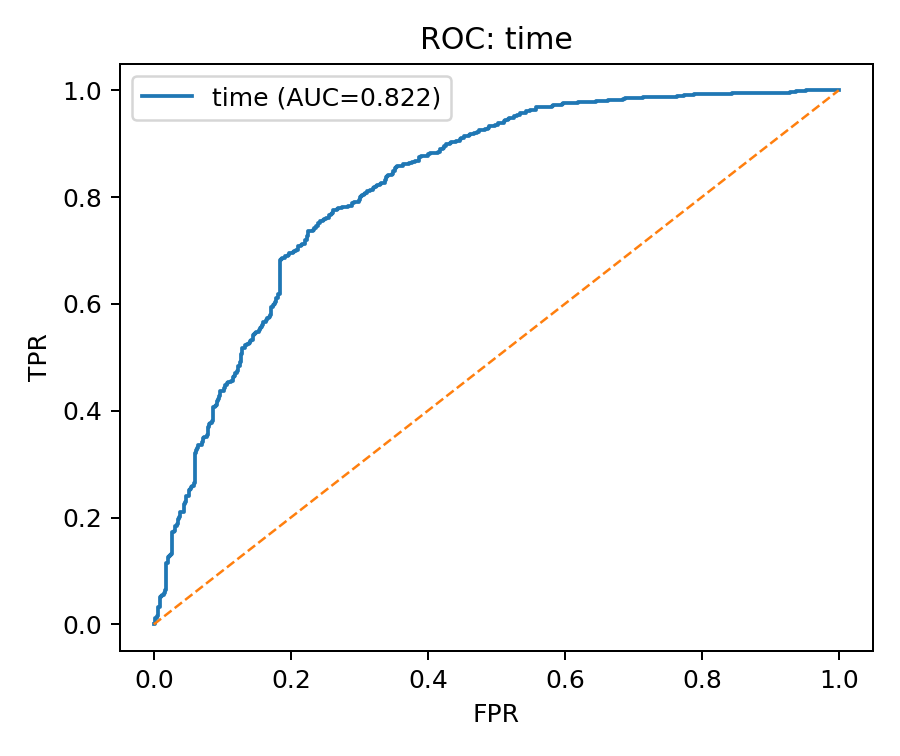
\includegraphics[width=0.45\linewidth]{images_in_paper/roc_time.png}
  \hfill
  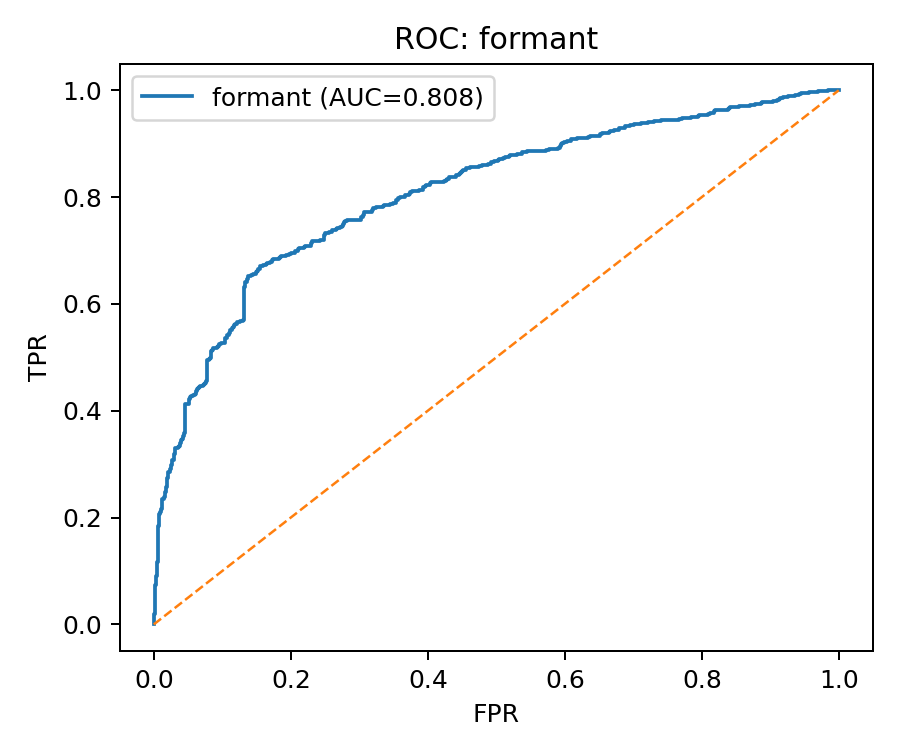
\includegraphics[width=0.45\linewidth]{images_in_paper/roc_formant.png}
  \caption{时域分支与 formant 分支 ROC 曲线。}
  \label{fig:roc}
\end{figure}

\end{frame}


\begin{frame}{量化分析结果:分支可分性指标对比}

\textbf{对比分析:}
\begin{itemize}
  \item 图~\ref{fig:branch_metrics} 展示各分支的 AUC、ACC 与 Fisher 比率;
  \item 时域与 formant 分支在三个指标上均占优;
  \item prosody 与 hjorth 分支指标普遍偏低,表明其独立判别能力有限;
  \item 说明融合决策阶段模型主要依赖结构性强、时频特征稳定的分支。
\end{itemize}
\end{frame}

\begin{frame}{量化分析结果:分支可分性指标对比}
\begin{figure}
  \centering
  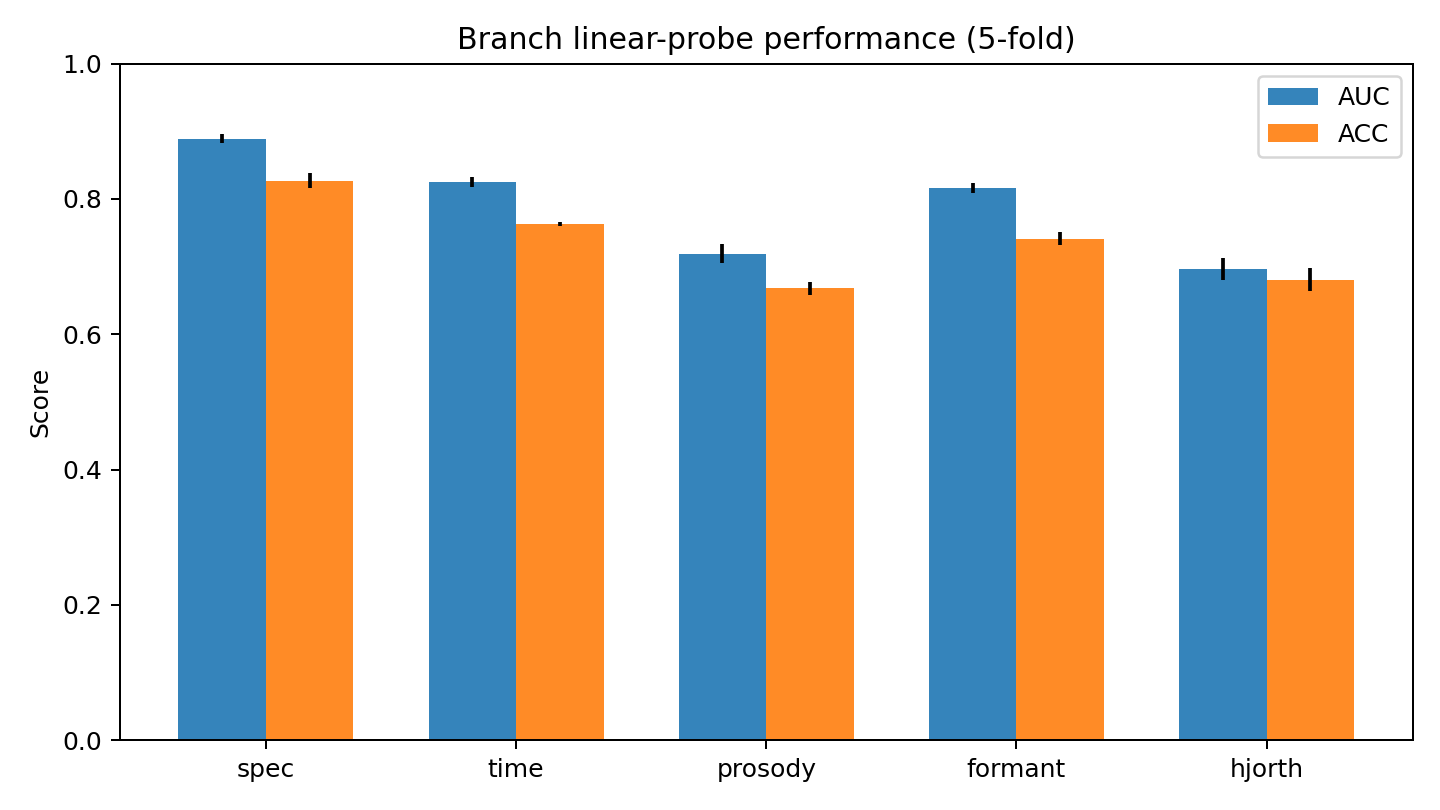
\includegraphics[width=0.32\linewidth]{images_in_paper/branch_metrics_auc_acc.png}
  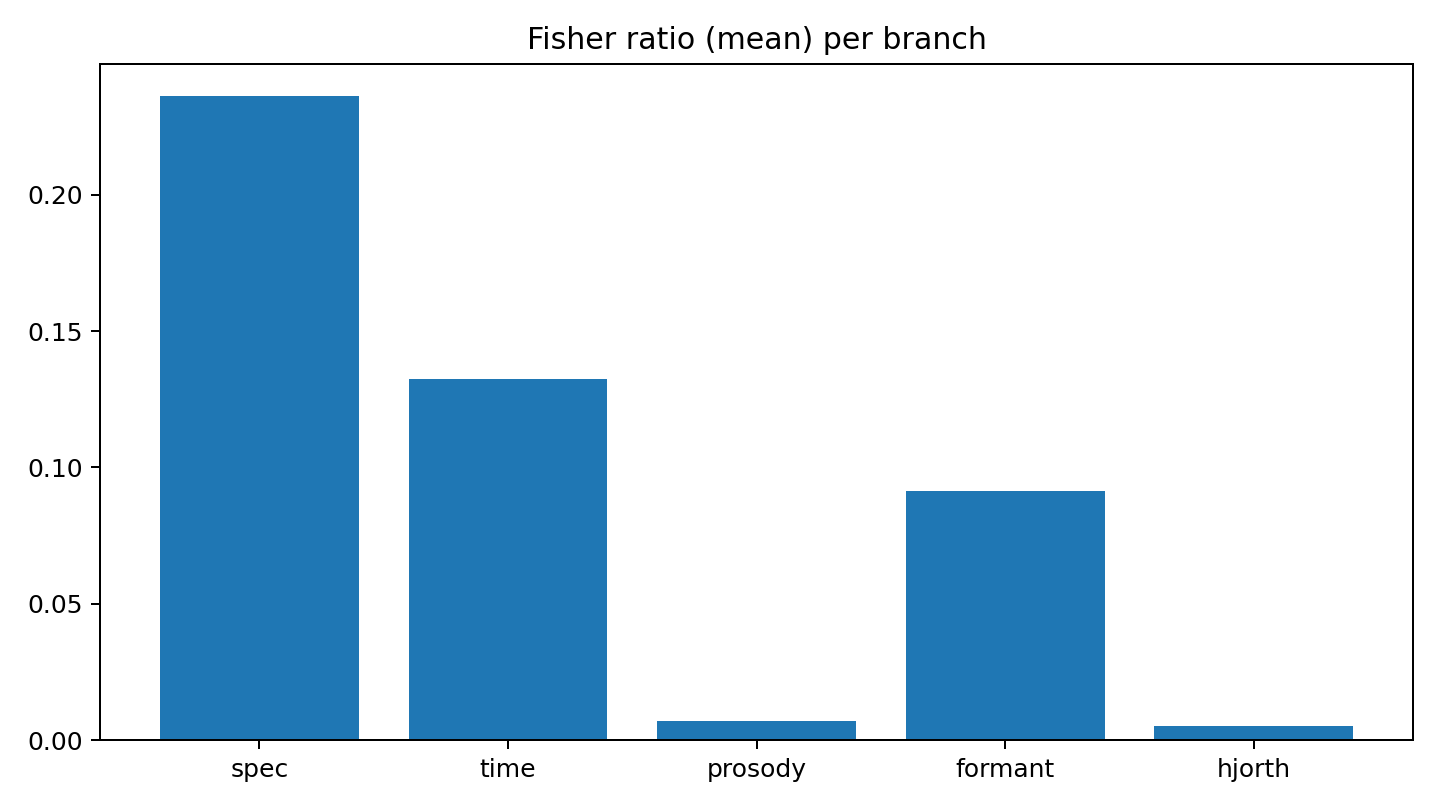
\includegraphics[width=0.32\linewidth]{images_in_paper/branch_fisher.png}
  \caption{分支可分性定量指标:AUC/ACC(左)、Fisher 比率(右)。}
  \label{fig:branch_metrics}
\end{figure}
\end{frame}

\begin{frame}{量化分析结果:分支可分性指标对比}
\textbf{总结:}
当时域包络或共振峰结构被扰动时,  
模型主分类概率显著向“非 AI”区域偏移,验证了模型对这些关键声学特征的依赖性。
\end{frame}

% \begin{frame}{偏差与失败模式}
% \textbf{观察:}
% \begin{itemize}
%   \item 自然环境纹理(雨声、林声、城市公园等)在排序表中获得较低 AI 概率;
%   \item 模型对\emph{非乐音 / 非稳态}素材存在天然“真值”偏好;
%   \item 该偏差可能源于训练集分布不均:
%         音乐性与稳态谐波成分占比更高。
% \end{itemize}
%
% \vspace{0.6em}
% \textbf{启示:}
% \begin{itemize}
%   \item 通过\textbf{轻度压缩 + 全通相位}改变瞬态,
%         或\textbf{小幅峰值 EQ} 微移 formant,
%         可在不改变主观听感的前提下显著提高“过检”概率;
%   \item 说明模型在\textbf{稳态性}与\textbf{谐波结构}上的依赖导致偏差。
% \end{itemize}
%
% \end{frame}


\begin{frame}{模型优缺点}

\small
\paragraph{模型优点}
\begin{itemize}
  \item 融合层充分利用多源信息的互补性;
  \item 具有较好的鲁棒性,即使在分类器受到干扰的情况下,基于多分枝独立判断的加权评分仍然稳健
  \item 特征提取部分与分类器解耦、各分支之间解耦,模型扩展性强
  \item 模型轻量、计算成本低、可实时检测并跨平台部署。
\end{itemize}

\vspace{0.6em}
\paragraph{模型不足}
\begin{itemize}
  \item 特征融合层为简单拼接,缺乏对分支质量的动态自适应;
  \item 训练数据覆盖有限,对新风格或新算法生成的音乐适配性不足。
\end{itemize}

\end{frame}

\begin{frame}{改进思路}
\begin{enumerate}
  \item \textbf{解耦式分支扩展(Plug-in):}  
        利用当前架构“特征提取与分类器解耦、分支间解耦”的优势,
        一方面可以设计可热插拔的分支接口,便于不断添加新的分支;另一方面,可以换用其他比MLP更强的分类器来进行的最终的分类
  \item \textbf{数据层面优化:}  
        通过扩充多样化的训练样本缓解数据覆盖不足问题,增加不同风格、
        不同生成算法的 AI 音频,并在训练中引入动态压缩、全通相位扰动、
        微小时间伸缩等数据增强手段,以提升模型的泛化与鲁棒性。
  \item \textbf{结构层面优化:}  
        在多分支融合层中引入一致性正则或
        分支级 dropout 机制,以抑制单一分支对判决的主导作用,
        促使模型在多个分支间学习到更加均衡的判别信息。
  \item \textbf{自适应机制引入:}  
        将静态拼接式融合改为基于注意力或门控机制的动态加权,
        使融合层能根据分支质量自适应分配权重,从而提升整体决策的灵活性与解释性。
\end{enumerate}
\end{frame}
% \begin{frame}{模型推广与应用前景}
%
% \small
% \paragraph{框架扩展性}
% \begin{itemize}
%   \item 多分支结构可灵活替换或新增特征分支;
%   \item 语音伪造检测:加入相位一致性特征;
%   \item 环境音识别:引入空间声学特征;
%   \item 可结合自编码器进行自监督预训练,提高低资源场景性能。
% \end{itemize}
%
% \vspace{0.6em}
% \paragraph{混合检测思路}
% \begin{itemize}
%   \item 将本模型与传统机器学习(如 XGBoost、SVM)特征融合;
%   \item 构建多模态、多尺度检测框架;
%   \item 推广至更多 AI 音频内容安全与生成溯源领域。
% \end{itemize}
%
% \vspace{0.8em}
% \centering
% {\Large \textbf{→ 面向开放域、低资源与实时检测的统一声学特征框架}}
% \end{frame}

\begin{frame}[standout]
  谢谢大家!
\end{frame}
% \appendix
\end{document}
